%%%%%%%%%%%%%%%%%%%%%%%%%%%%%%%%%%%%%%%%%%%%%%%%%%%%%%%%%%%%%%%%%%%%%%%%%%%%%%%%
%%                                                                            %%
%%  EXAMPLE                                                                   %%
%%                                                                            %%
%%%%%%%%%%%%%%%%%%%%%%%%%%%%%%%%%%%%%%%%%%%%%%%%%%%%%%%%%%%%%%%%%%%%%%%%%%%%%%%%

% [x] Beispiel vorstellen
% [x] Mapping beschreiben

\section{Example}
\label{sec:example}

% Einleitung
In this section we will exemplify several aspects of the mapping by means of a
simple example, as shown in Figure~\ref{fig:example}.

% Prozessdiagramm
\begin{figure*}
	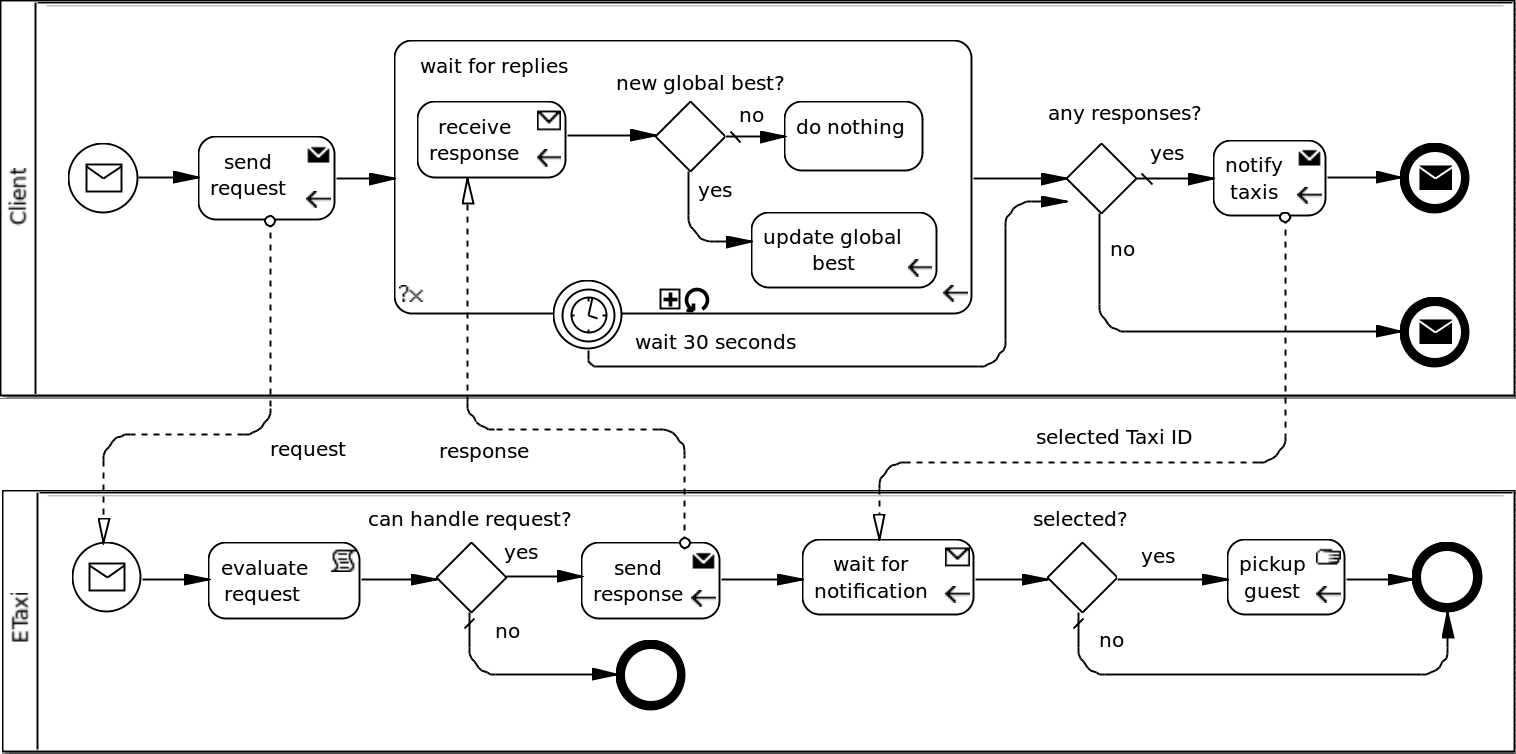
\includegraphics[width=\textwidth]{img/example.png}
	\caption{Example: Taxi Request Service}
	\label{fig:example}
\end{figure*}

% Beschreibung des Beispielprozesses
The BPMN diagram consists of two Pools, each representing an agent role: Client,
and E-Taxi.  The Client's process starts by broadcasting a request (customer ID,
location, destination, desired time of arrival) to all available E-Taxis, which
evaluate the request and decide whether they can handle it, in which case they
send a response (taxi ID, estimated time of arrival, price).  The Client enters
a looping subprocess, listening to responses and memorizing the best response,
until after 30 seconds the subprocess is interrupted by the attached timer event.
The Client then sends notifications to the responding E-Taxis, and the selected
E-Taxi prepares to pick up the guest.  Note that the several properties (variables)
and assignments are not visualized in the diagram.

% Sourcecode-Listing
The resulting Agent Bean for the Client role is shown in Listing~\ref{lst:example1},
slightly shortened to improve readability and to better fit into this paper.

\lstinputlisting[language=Java, caption=Generated Agent Bean: Client\_requestTaxi,
                 label=lst:example1]{img/example1.java}

% Beschreibung der Haupt-Klasse
As can be seen, the control-flow of the process is reflected in the workflow-method
\verb_requestTaxi()_, which is also exposed as a JIAC Action, or Service.  The
workflow-method is dominated by the threads for running the subprocess and the
attached event handler, but also contains an if-else-statement for the Gateway
at the end of the process.  The activities \emph{send request} and \emph{notify
taxis} are mapped to two similar methods for sending a JIAC message to the
specified broadcast message group.

% Beschreibung der inneren Klassen
The subprocess is mapped to an inner class, also forming a new variable scope for
the properties of the subprocess.  It features another workflow-method and several
activity-methods, most notably the \emph{receive responses} method, in which the
Client joins the specified message group and checks its memory for accordant
messages.  The subprocess is executed as a thread which is to be interrupted by
the event handler thread.  Both are shown in Listing~\ref{lst:example2}.

\lstinputlisting[language=Java, caption=Inner Classes for Subprocess and Event Handler,
                 label=lst:example2]{img/example2.java}

